\section{Analyse des résultats}\label{sec:analyse-des-resultats}
Premièrement, on constate dans la table~\ref{tab:eta-val} que plus la bille est petite, plus son
temps de chute est lent (la valeur de $\eta$ obtenue pour la bille 1 [mm] est entre les deux autres),
et donc plus la mesure est précise ;
néanmoins, cette précision peut en partie être contrebalancée par celle dans la mesure de la bille qui
sera moindre.
On constate ça également avec les graphes et tables de vitesses qui montrent que plus la bille est petite,
plus elle va lentement. \\
Ensuite, on constate que les simulations correspondent bien aux mesures, en comparant
les vitesses dans la table~\ref{tab:vitesse} avec les graphes des figures~\ref{fig:ray1_it}, ~\ref{fig:ray2_it} et~\ref{fig:ray3_th} : les valeurs de la table correspondent à peu près (à cause
des arrondis sur $\eta$) à l'endroit où convergent/tendent les graphes de vitesse.
De plus, cela confirme le concept de vitesse limite que nous laissait percevoir le modèle des forces :
la force pesante étant plus grande que la force d'Archimède et les deux étant constante ;
de fait, seul la force de frottement va varier en s'opposant au mouvement de la bille qui coule.
Pour conclure, lorsque la somme des forces est nul, la vitesse limite est atteinte.
Comme on le voit sur les graphes, il ne faut pas longtemps à la bille pour y arriver.
\\
Toujours en parlant de fonction, on voit que la résolution "litérale" correspond à la méthode
itérative.
En effet, la figure~\ref{fig:ray3_th} est la même que celle~\ref{fig:ray3_it}. \\
De plus, cette fonction théorique nous indique que la vitesse est une fonction exponentielle du
temps, et de fait on peut connaitre la fonction de l'accélération $a(t)= \frac{d}{dt} \left( \frac{A}{B}+c \cdot
e^{-B\cdot t} \right)= -B\cdot c\cdot e^{-B \cdot t} $ et la fonction de la position
$ x(t) = \int \frac{A}{B}+c \cdot e^{-B\cdot t} dt = \frac{A \cdot t - c \cdot e^{-B\cdot t}}{B} + c_{1} $
où $c$ est la constante définie dans la section~\ref{subsec:simulations} et $c_{1}$ une autre constante
liée à l'intégrale, que l'on peut calculer de la même manière que $c$ en connaissant $x_{0}$ dans ce cas.\\
Le diagramme en figure~\ref{fig:densplot} illustre aussi la convergence quelle que soit la vitesse
initiale (les zones violettes sont celles avec le moins de points et plus il y en a, plus ça tend vers
le jaune). \\
Finalement, on peut grâce à la valeur d'$\eta$ trouvée estimer la concentration en glycérine de la
solution utilisée via la table~\ref{tab:table-viscu} : $\sim 85-90 \%$.

\begin{table}[H]
    \centering
    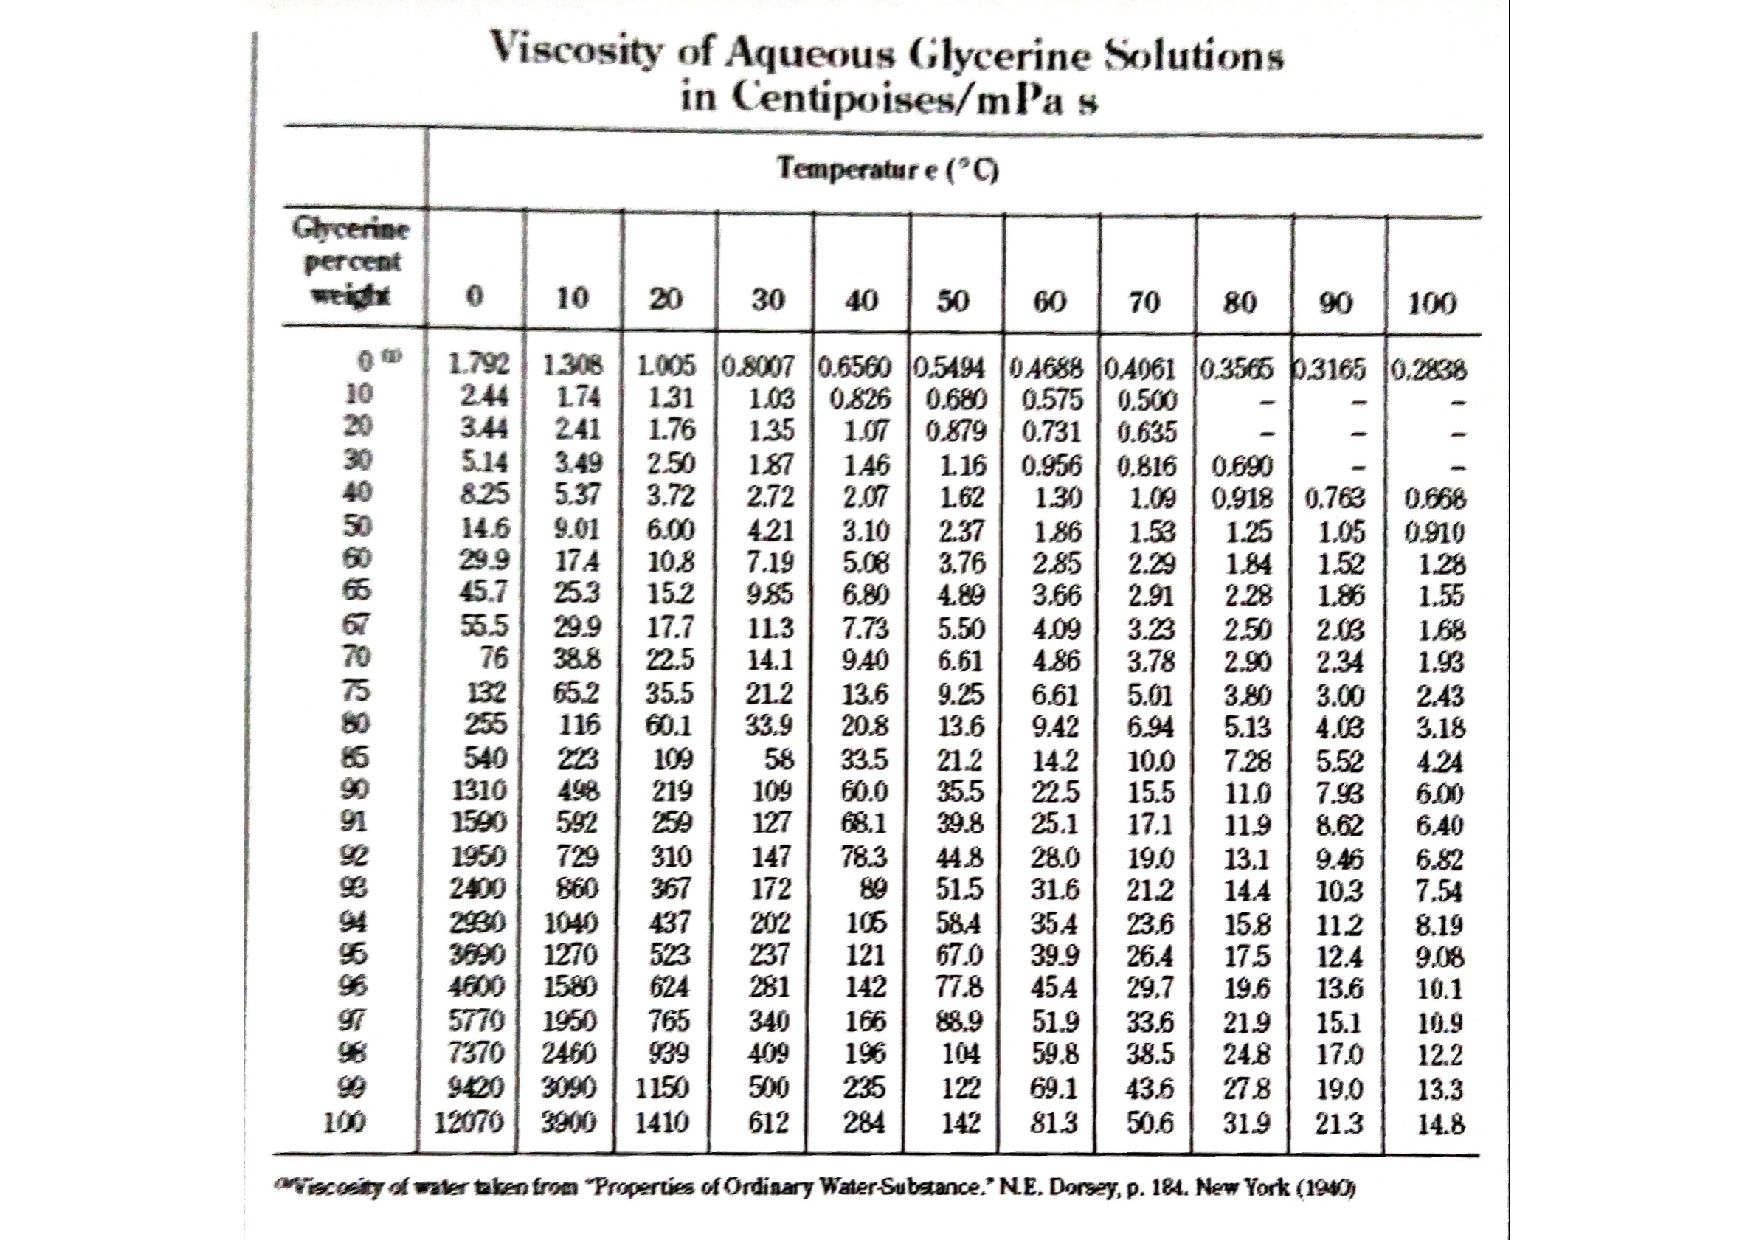
\includegraphics[scale=0.5]{graph/table-viscu}
    \caption{Viscosité d'un mélange eau-glycérine en fonction de sa concentration}
    \label{tab:table-viscu}
\end{table}